
%\chapter{Corrections des Travaux Dirigés}

\section{Corrélations quantiques}

\subsection{Inégalités de Bell avec des photons}

\begin{enumerate}
 \item Évaluons les vecteur $\ket{\theta\theta_{\bot}}$ et
$\ket{\theta_{\bot}\theta}$:
 \begin{subequations}
 \begin{align}
\ket{\theta\theta_{\bot}} & =(\cos\theta\ket{x}+\sin\theta\ket{y})
(-\sin\theta\ket{x}+\cos\theta\ket{y})\\
& = -\sin\theta\cos\theta\ket{xx}+\cos^2\theta\ket{xy}-\sin^2\theta\ket{yx}+
\sin\theta\cos\theta\ket{yy},\\
\ket{\theta_{\bot}\theta} &=-\sin\theta\cos\theta\ket{xx}+\cos^2\theta\ket{yx}
-\sin^2\theta\ket{xy}+\sin\theta\cos\theta\ket{yy}.
 \end{align}
On en déduit
\begin{equation}
\ket{\Psi}=\frac{1}{\sqrt{2}}(\ket{\theta\theta_{\bot}}-\ket{\theta_{\bot}
\theta})=\frac{1}{\sqrt{2}}(\ket{xy}-\ket{yx}).
\end{equation}
 \end{subequations}

\item Pour le photon (1),
 \begin{subequations}
\begin{equation}
 \ket{x}=\frac{1}{\sqrt{2}}(-\ket{D}+\ket{G}),\,\ket{y}=\frac{i}{\sqrt{2}}(\ket{
D}+\ket{G}),
\end{equation}
et pour le photon (2), il suffit de changer $\ket{y}$ en $-\ket{y}$,
\begin{equation}
 \ket{x}=\frac{1}{\sqrt{2}}(-\ket{D}+\ket{G}),\,\ket{y}=-\frac{i}{\sqrt{2}}(\ket
{D}+\ket{G}),
\end{equation}
et on trouve, pour des photons ayant une direction de propagation opposée,
\begin{equation}
\begin{split}
 \ket{\Psi} &=-\frac{i}{\sqrt{2}}(-\ket{DD}-\ket{DG}+\ket{GD}-\ket{DD}+\ket{DG}
-\ket{GD}+\ket{GG})\\
 &=\frac{i}{\sqrt{2}}(\ket{DD}-\ket{GG}).
\end{split}
\end{equation}
 \end{subequations}

\item Puisque $\mathcal{P}_D=\ket{D}\bra{D}$ et $\mathcal{P}_G=\ket{G}\bra{G}$,
 \begin{subequations}
\begin{equation}
\begin{split}
\Sigma_{z}^(\dag)&=(\ket{D}\bra{D}-\ket{G}\bra{G})^{\dag}=\frac{1}{2}[(\ket{x}
+i\ket{y })(\bra{x}-i\bra{y})-(\ket{x}-i\ket{y})(\bra{x}+i\bra{y})]^{\dag}\\
&=\ket{D}\bra{D}-\ket{G}\bra{G}=\Sigma_{z}.
\end{split}
\end{equation}
D'autre part,
\begin{equation}
 \Sigma_{z}\ket{D}=+\ket{D},\,\Sigma_{z}\ket{G}=-\ket{G}.
\end{equation}
Compte tenu de ce qui précède,
\begin{equation}
 \Sigma_{z}\ket{\Psi}=\frac{i}{\sqrt{2}}(\ket{DD}-\ket{GG})=\ket{\Psi},
\end{equation}
\end{subequations}
c'est-à-dire que $\ket{\Psi}$ est invariant par rotation autour de $Oz$.

\item En raison cette invariance, les probabilités $\texttt{p}(\alpha,\beta)$
ne dépendent que de la différence des angles $\phi=\beta-\alpha$. On peut donc
choisir $\hat{n}_{\alpha}$ suivant l'axe $Ox$ et $\hat{n}_{\beta}$ dans
le plan $xOy$ et faisant un angle $\phi=\beta-\alpha$ avec l'axe $Ox$.
\begin{enumerate}
\item
\begin{itemize}
 \item L'amplitude de probabilité pour que le photon soit projeté dans l'état
 \begin{subequations}
  \begin{equation}
  \ket{x}\otimes\ket{\phi}=\cos\phi\ket{xx}+\sin\phi\ket{xy},
 \end{equation}
 est
\begin{equation}
\mathtt{a}_{++}(\alpha,\beta)=\frac{1}{\sqrt{2}}(\cos\phi\bra{xx}+
\sin\phi\bra{xy})(\ket{xy} -\ket{yx})=\frac{1}{\sqrt{2}}\sin\phi,
\end{equation}
et donc
\begin{equation}
 \texttt{p}{++}(\alpha,\beta)=\frac{1}{2}\sin^2\phi.
\end{equation}
\end{subequations}
\item Par symétrie dans l'échange $x\leftrightarrow\mathtt{W} y$ on trouve
\begin{equation}
 \texttt{p}{--}(\alpha,\beta)=\texttt{p}{++}(\alpha,\beta)=\frac{1}{2}
\sin^2\phi.
\end{equation}
\item Comme la somme de toutes les probabilités doit donner $1$,
\begin{equation}
 \texttt{p}_{+-}(\alpha,\beta)=\texttt{p}_{-+}(\alpha,\beta)=\frac{1}{2}
\cos^2\phi.
\end{equation}
On en déduit
\begin{equation}
\begin{split}
E(\alpha,\beta)&=[\texttt{p}_{++}(\alpha,\beta)+\texttt{p}_{--}(\alpha,\beta)]-[
\texttt{p}_{+-} (\alpha,\beta)+\texttt{p}_{+-}(\alpha,\beta)]\\
&=\sin^2\phi-\cos^2\phi=-\cos2\phi.
\end{split}
\end{equation}
\end{itemize}
\item Dans la cas du spin-$\frac{1}{2}$, $E(\alpha,\beta)=-\cos\phi$. Ainsi,
pour les photons de spin 1, il faut utiliser des angles moitié de ceux du
spin-$\frac{1}{2}$.
\end{enumerate}
\item On trouve sans difficulté question
 \begin{equation}
\ket{\Phi}=\frac{1}{\sqrt{2}}(\ket{xy}-\ket{yx})=\frac{1}{\sqrt{2}}
(\ket{\theta\theta}-\ket{\theta_{\bot}\theta_{\bot}})=\frac{1}{\sqrt{2}}
(\ket{DD}+\ket{GG}).
\end{equation}
L'application de $\Sigma_z$ montre que l'état $\ket{\Phi}$ est de moment
angulaire nul.
\end{enumerate}

\subsection{Distribution quantique des clefs 1}

\subsubsection{BB4 sans espion}

\begin{enumerate}
\item \textbf{ Phase Envoie}.

{\footnotesize {
\begin{tabular}
[c]{|l|l|l||l|l|l|}\hline
\rowcolor[gray]{0.8}\textbf{A envoie} & \textbf{B mesure et trouve} &
\textbf{Probabilité} & \textbf{A envoie} & \textbf{B mesure et trouve} &
\textbf{Probabilité}\\\hline
$\ket{0_z} $ & $Z\rightarrow\mathtt{W}\ket{0_z}$ & $1$ & $\ket{0_x} $ &
$Z\rightarrow\mathtt{W}\ket{0_z} $ & $\frac{1}{2}$\\\hline
$\ket{0_z} $ & $Z\rightarrow\mathtt{W}\ket{1_z}$ & $0$ & $\ket{0_x} $ &
$Z\rightarrow\mathtt{W}\ket{1_z} $ & $\frac{1}{2}$\\\hline
$\ket{0_z} $ & $X\rightarrow\mathtt{W}\ket{0_x}$ & $\frac{1}{2}$ & $\ket{0_x} $
& $X\rightarrow\mathtt{W}\ket{0_x} $ & $1$\\\hline
$\ket{0_z} $ & $X\rightarrow\mathtt{W}\ket{1_x}$ & $\frac{1}{2}$ & $\ket{0_x} $
& $X\rightarrow\mathtt{W}\ket{1_x} $ & $0$\\\hline\hline
$\ket{1_z} $ & $Z\rightarrow\mathtt{W}\ket{0_z}$ & $0$ & $\ket{1_x} $ &
$Z\rightarrow\mathtt{W}\ket{0_z} $ & $\frac{1}{2}$\\\hline
$\ket{1_z} $ & $Z\rightarrow\mathtt{W}\ket{1_z}$ & $1$ & $\ket{1_x} $ &
$Z\rightarrow\mathtt{W}\ket{1_z} $ & $\frac{1}{2}$\\\hline
$\ket{1_z} $ & $X\rightarrow\mathtt{W}\ket{0_x}$ & $\frac{1}{2}$ & $\ket{1_x} $
& $X\rightarrow\mathtt{W}\ket{0_x} $ & $0$\\\hline
$\ket{1_z} $ & $X\rightarrow\mathtt{W}\ket{1_x}$ & $\frac{1}{2}$ & $\ket{1_x} $
& $X\rightarrow\mathtt{W}\ket{1_x} $ & $1$\\\hline
\end{tabular}
}}

\item Il est clair qu'après la phase \textbf{sifting}, Alice et Bob partagent
une liste identique de bits secrets. Ces bits sont secrets car ils n'ont pas
été communiqué en public. Seule les bases ont été communiqué et pas les bits.
\end{enumerate}

\subsubsection{BB4 avec espion}

\begin{enumerate}
\item \textbf{Attaque d'Eve.} On note sur le tableau ci-dessous qu'Alice et
Bob n'ont pas le même bit en présence de l'attaque d'Eve, malgré le fait
qu'ils ont effectué les mesures dans la même base.

{\footnotesize {
\begin{tabular}
[c]{|p{1.1cm}|p{2cm}|p{2.1cm}|l||p{1.1cm}|p{2cm}|p{2.1cm}|l|}\hline
\rowcolor[gray]{0.8}\textbf{A envoie} & \textbf{E mesure et trouve} &
\textbf{B mesure et trouve} & \textbf{Proba} & \textbf{A envoie} &
\textbf{E mesure et trouve} & \textbf{B mesure et trouve} &
\textbf{Proba}\\\hline
\multicolumn{1}{|l|}{$\ket{0_z} $} &
\multicolumn{1}{|c|}{$Z\rightarrow\mathtt{W}\ket{0_z} $} &
\multicolumn{1}{|c|}{$Z\rightarrow\mathtt{W}\ket{0_z} $} & $\frac
{1}{2}$ & \multicolumn{1}{||l|}{$\ket{1_z} $} &
\multicolumn{1}{|c|}{$Z\rightarrow\mathtt{W}\ket{0_z} $} &
\multicolumn{1}{|c|}{$Z\rightarrow\mathtt{W}\ket{0_z} $} &
$0$\\\hline
\multicolumn{1}{|l|}{$\ket{0_z} $} &
\multicolumn{1}{|c|}{$Z\rightarrow\mathtt{W}\ket{0_z} $} &
\multicolumn{1}{|c|}{$Z\rightarrow\mathtt{W}\ket{1_z} $} & $0$ &
\multicolumn{1}{||l|}{$\ket{1_z} $} &
\multicolumn{1}{|c|}{$Z\rightarrow\mathtt{W}\ket{0_z} $} &
\multicolumn{1}{|c|}{$Z\rightarrow\mathtt{W}\ket{1_z} $} &
$0$\\\hline
\multicolumn{1}{|l|}{$\ket{0_z} $} &
\multicolumn{1}{|c|}{$Z\rightarrow\mathtt{W}\ket{1_z} $} &
\multicolumn{1}{|c|}{$Z\rightarrow\mathtt{W}\ket{0_z} $} & $0$ &
\multicolumn{1}{||l|}{$\ket{1_z} $} &
\multicolumn{1}{|c|}{$Z\rightarrow\mathtt{W}\ket{1_z} $} &
\multicolumn{1}{|c|}{$Z\rightarrow\mathtt{W}\ket{0_z} $} &
$0$\\\hline
\multicolumn{1}{|l|}{$\ket{0_z} $} &
\multicolumn{1}{|c|}{$Z\rightarrow\mathtt{W}\ket{1_z} $} &
\multicolumn{1}{|c|}{$Z\rightarrow\mathtt{W}\ket{1_z} $} & $0$ &
\multicolumn{1}{||l|}{$\ket{1_z} $} &
\multicolumn{1}{|c|}{$Z\rightarrow\mathtt{W}\ket{1_z} $} &
\multicolumn{1}{|c|}{$Z\rightarrow\mathtt{W}\ket{1_z} $} & $\frac
{1}{2}$\\\hline
\multicolumn{1}{|l|}{$\ket{0_z} $} &
\multicolumn{1}{|c|}{$X\rightarrow\mathtt{W}\ket{0_x} $} &
\multicolumn{1}{|c|}{$Z\rightarrow\mathtt{W}\ket{0_z} $} & $\frac
{1}{8}$ & \multicolumn{1}{||l|}{$\ket{1_z} $} &
\multicolumn{1}{|c|}{$X\rightarrow\mathtt{W}\ket{0_x} $} &
\multicolumn{1}{|c|}{$Z\rightarrow\mathtt{W}\ket{0_z} $} & $\frac
{1}{8}$\\\hline
\multicolumn{1}{|l|}{$\ket{0_z} $} &
\multicolumn{1}{|c|}{$X\rightarrow\mathtt{W}\ket{0_x} $} &
\multicolumn{1}{|c|}{$Z\rightarrow\mathtt{W}\ket{1_z} $} & $\frac
{1}{8}$ & \multicolumn{1}{||l|}{$\ket{1_z} $} &
\multicolumn{1}{|c|}{$X\rightarrow\mathtt{W}\ket{0_x} $} &
\multicolumn{1}{|c|}{$Z\rightarrow\mathtt{W}\ket{1_z} $} & $\frac
{1}{8}$\\\hline
\multicolumn{1}{|l|}{$\ket{0_z} $} &
\multicolumn{1}{|c|}{$X\rightarrow\mathtt{W}\ket{1_x} $} &
\multicolumn{1}{|c|}{$Z\rightarrow\mathtt{W}\ket{0_z} $} & $\frac
{1}{8}$ & \multicolumn{1}{||l|}{$\ket{1_z} $} &
\multicolumn{1}{|c|}{$X\rightarrow\mathtt{W}\ket{1_x} $} &
\multicolumn{1}{|c|}{$Z\rightarrow\mathtt{W}\ket{0_z} $} & $\frac
{1}{8}$\\\hline
\multicolumn{1}{|l|}{$\ket{0_z} $} &
\multicolumn{1}{|c|}{$X\rightarrow\mathtt{W}\ket{1_x} $} &
\multicolumn{1}{|c|}{$Z\rightarrow\mathtt{W}\ket{1_z} $} & $\frac
{1}{8}$ & \multicolumn{1}{||l|}{$\ket{1_z} $} &
\multicolumn{1}{|c|}{$X\rightarrow\mathtt{W}\ket{1_x} $} &
\multicolumn{1}{|c|}{$Z\rightarrow\mathtt{W}\ket{1_z} $} & $\frac
{1}{8}$\\\hline
\end{tabular}
} }

\item Bien qu'Alice et Bob utilisent la même base, ils n'ont pas forcement le
même bit (car on a nulle part ou la probabilité est égale à $1$). Ceci est dû
au faite qu'Alice et Bob utilisent deux bases. En effet, s'ils utilisaient une
seule base, Eve en utilisant la même base aurait laissé le photon après sa
mesure dans le même état de polarisation qu'Alice: \emph{la mesure effectuée
par Eve ne perturbe pas le système} et son intrusion ne sera jamais détectée
par Alice et Bob.

\item Dans le même base, et en absence d'Eve, des bits (résultats) d'Alice et
Bob sont identiques. Donc si \textbf{une seule} mesure dans cette base commune
est différente, la présence d'Eve est certaine?
\end{enumerate}

\subsection{Distribution quantique des clefs 2}

\begin{enumerate}
\item
\begin{enumerate}
 \item 

\begin{itemize}
 \item Vecteurs propres. À partir de $\ket{u\pm}=R_y(\theta)\ket{z\pm}$, avec 
$R_y=\begin{pmatrix}\cos\frac{\theta}{2} & -\sin\frac{\theta}{2}\\
                   \sin\frac{\theta}{2} & \cos\frac{\theta}{2}\end{pmatrix}$, 
on trouve sans peine
              \begin{equation}
               \ket{u+}=\begin{pmatrix}
                         \cos\frac{\theta}{2}\\\sin\frac{\theta}{2}
                        \end{pmatrix},\,
               \ket{u-}=\begin{pmatrix}
                         -\sin\frac{\theta}{2}\\\cos\frac{\theta}{2}
                        \end{pmatrix}.
              \end{equation}

\item Probabilités. Compte tenu de 
$\mathcal{P}^{\pm}_{u\leftarrow z+} 
=|\langle u\pm\ket{z+}|^2$, on a
\begin{equation}
\mathcal{P}^{+}_{u\leftarrow z+}(\theta)=\cos^2\frac{\theta}{2}\,\,\mathcal{P}^ 
{-}_{u\leftarrow z+}(\theta)=\sin^2\frac{\theta}{2}.
     \end{equation}
Et on vérifie bien que $\mathcal{P}^{+}_{u\leftarrow z+}(\theta) 
+\mathcal{P}^{-}_{u\leftarrow z+}(\theta)=1$.
       \end{itemize}

\item En vertu du principe de réduction du paquet d'onde:
$+\frac{\hbar}{2}\,\rightarrow\,\ket{u+}$ et
$-\frac{\hbar}{2}\,\rightarrow\,\ket{u-}$.
\end{enumerate}

\item
\begin{enumerate}
 \item \begin{itemize}
        \item Mesure de $u$: $+\frac{\hbar}{2}$. Compte tenu de 
$\mathcal{P}^{\pm}_{z\leftarrow u+} =|\langle z\pm\ket{u+}|^2$, on a
\begin{equation}
\mathcal{P}^{+}_{z\leftarrow u+}(\theta)=\cos^2\frac{\theta}{2}\,\,\mathcal 
{P}^{-}_{z\leftarrow u+}(\theta)=\sin^2\frac{\theta}{2}.
     \end{equation}

     \item Mesure de $u$: $-\frac{\hbar}{2}$. Compte tenu de 
$\mathcal{P}^{\pm}_{z\leftarrow u-} =|\langle z\pm\ket{u-}|^2$, on a
\begin{equation}
\mathcal{P}^{+}_{z\leftarrow u-}(\theta)=\sin^2\frac{\theta}{2}\,\,\mathcal 
{P}^{-}_{z\leftarrow u-}(\theta)=\cos^2\frac{\theta}{2}.
     \end{equation}
       \end{itemize}

\item On trouve $s_z=+\frac{\hbar}{2}$ avec la probabilité
\begin{equation}
\mathcal{P}^{+}_{u\leftarrow z+}(\theta)\mathcal{P}^{+}_{z\leftarrow u+} 
=\cos^4\frac{\theta}{2},\,\, 
 \mathcal{P}^{-}_{u\leftarrow z-}(\theta)\mathcal{P}^{+}_{z\leftarrow u-} 
=\sin^4\frac{\theta}{2},                           
\end{equation}
soit
\begin{equation}
  \mathcal{P}_{++}(\theta) =\cos^4\frac{\theta}{2}+\sin^4\frac{\theta}{2} 
=\frac{1}{2}(1+\cos^2\theta). 
\end{equation}

\item Les résultats intermédiaires sont inversés, mais la probabilité est la
même
\begin{equation}
 \mathcal{P}_{--}(\theta)=\frac{1}{2}(1+\cos^2\theta).
\end{equation}

\end{enumerate}

\item 
\begin{enumerate}
 \item En vertu de
 \begin{equation}
  \ket{x\pm}=\frac{1}{\sqrt{2}}(\ket{z+}\pm\ket{z-}),
 \end{equation}
 \begin{align}
 \ket{\Sigma}&=\frac{1}{\sqrt{2}}(\ket{x+x+}+\ket{x-x-}),\label{eq:Sigma1}\\
 &=\frac{1}{2\sqrt{2}}\lbrace(\ket{z+}+\ket{z-})\otimes(\ket{z+}+\ket{z-}
)+(\ket{ z+ } -\ket{z-})\otimes(\ket{z+}-\ket{z-})\rbrace\\
&=\frac{1}{\sqrt{2}}(\ket{z+z+}+\ket{z-z-}).\label{eq:Sigma2}
\end{align}

\item 
\begin{enumerate}
 \item En vertu de (\ref{eq:Sigma1}) ou (\ref{eq:Sigma2}), Alice trouve
$\pm\frac{\hbar}{2}$ avec une probabilité $p=+1/2$ dans chaque cas. En effet,
\begin{align}
 \mathcal{P}^{+}_{u_a\leftarrow\Sigma_a}(0) & =\frac{1}{2}(1+0)=\frac{1}{2},\,\,
 \mathcal{P}^{-}_{u_a\leftarrow\Sigma_a}(0)=\frac{1}{2}(0+1)\frac{1}{2},\\
 \mathcal{P}^{+}_{u_a\leftarrow\Sigma_a}(\frac{\pi}{2}) & 
=\frac{1}{2}(\frac{1}{2}+\frac{1}{2})=\frac{1}{2},\,\,
\mathcal{P}^{-}_{u_a\leftarrow\Sigma_a}(\frac{\pi}{2})=\frac{1}{2}(\frac{1}{2}
+\frac{1}{2})=\frac{1}{2}.
\end{align}

\item Tout résultat de mesure $b$ fera intervenir des valeurs moyennes du type
$\mathbb{I}_a\otimes\mathtt{B}_b$. Par exemple
\begin{equation}
  \bra{z+z+}\mathbb{I}_a\otimes\mathtt{B}_b\ket{z+z+} =\langle z+\ket{z+} 
\bra{z+}\mathtt{B}_b\ket{z+}=\bra{z+}\mathtt{B}_b\ket{z+}
\end{equation}
et donc l'état $a$ n'intervient pas.
\end{enumerate}

\item Résultats des mesures de Bob et probabilités (sans espion).
\begin{center}
\begin{tabular}{|c|c|c|c|}\hline
$(\theta_a,\theta_b)$ & Résultat Alice & Résultat Bob & Probabilité\\\hline
$(0,0)$ & $+\frac{\hbar}{2}$ & $+\frac{\hbar}{2}$ & $1$\\\cline{2-4}
 & $-\frac{\hbar}{2}$ & $-\frac{\hbar}{2}$ & $1$\\\hline
$(0,\frac{\pi}{2})$ & $+\frac{\hbar}{2}$ & $\pm\frac{\hbar}{2}$ & 
$\frac{1}{2}$ chaque fois\\\cline{2-4}
 & $-\frac{\hbar}{2}$ & $\pm\frac{\hbar}{2}$ & $\frac{1}{2}$ chaque fois\\\hline
$(\frac{\pi}{2},0)$ & $+\frac{\hbar}{2}$ & $\pm\frac{\hbar}{2}$ & 
$\frac{1}{2}$ chaque fois\\\cline{2-4}
 & $-\frac{\hbar}{2}$ & $\pm\frac{\hbar}{2}$ & $\frac{1}{2}$ chaque fois\\\hline
$(\frac{\pi}{2},\frac{\pi}{2})$ & $+\frac{\hbar}{2}$ & $+\frac{\hbar}{2}$ & 
$1$\\\cline{2-4}
 & $-\frac{\hbar}{2}$ & $-\frac{\hbar}{2}$ & $1$\\\hline
\end{tabular}
\end{center}

Dans les cas $(0,0)$ et $(\frac{\pi}{2},\frac{\pi}{2})$, Alice et Bob trouvent
à coup sûr le même résultat avec la probabilité $1$.

\item 
\begin{enumerate}
 \item Résultats des mesures de Bob et probabilités (avec espion).
\begin{center}
\begin{tabular}{|c|c|c|c|c|}\hline
Résultat Alice & Résultat Espion & Probabilité& Résultat Bob & 
Probabilité\\\hline
 $+\frac{\hbar}{2}$ & $+\frac{\hbar}{2}$ & $\cos^2\frac{\theta_e}{2}$ & 
$+\frac{\hbar}{2}$ & $\cos^2\frac{\theta_e}{2}$\\\cline{4-5}
  &  &   & $-\frac{\hbar}{2}$ & $\sin^2\frac{\theta_e}{2}$\\\cline{2-5}
   & $-\frac{\hbar}{2}$ & $\sin^2\frac{\theta_e}{2}$ & 
$+\frac{\hbar}{2}$ & $\sin^2\frac{\theta_e}{2}$\\\cline{4-5}
  &  &   & $-\frac{\hbar}{2}$ & $\cos^2\frac{\theta_e}{2}$\\\hline
  $-\frac{\hbar}{2}$ & $+\frac{\hbar}{2}$ & $\sin^2\frac{\theta_e}{2}$ & 
$+\frac{\hbar}{2}$ & $\cos^2\frac{\theta_e}{2}$\\\cline{4-5}
  &  &   & $-\frac{\hbar}{2}$ & $\sin^2\frac{\theta_e}{2}$\\\cline{2-5}
   & $-\frac{\hbar}{2}$ & $\cos^2\frac{\theta_e}{2}$ & 
$+\frac{\hbar}{2}$ & $\sin^2\frac{\theta_e}{2}$\\\cline{4-5}
  &  &   & $-\frac{\hbar}{2}$ & $\cos^2\frac{\theta_e}{2}$\\\hline
\end{tabular}
\end{center}

\item Probabilité pour qu'Alice et Bob trouvent le même résultat.
\begin{equation}
\mathcal{P}_{++}(\theta_e)=\mathcal{P}_{--}(\theta_e)=\cos^4\frac{\theta_e}{2}
+\sin^4\frac{\theta_e}{2}=\frac{1}{2}(1+\cos^2\frac{\theta_e}{2}).
      \end{equation}


\item \label{item} Moyennes de la probabilité.
\begin{align}
&\frac{1}{2\pi}\int_0^{2\pi}\mathcal{P}(\theta_e)d\theta_e 
=\frac{1}{2\pi}\int_0^
{2\pi}\frac{1}{2}(1+\cos^2\frac{\theta_e}{2})d\theta_e
=\frac{1}{4\pi}\left[\frac{3}{2}\theta_e+\frac{1}{4}\sin2\theta_e\right]^{2\pi}
_0=\frac{3}{4},\\
& \frac{1}{2}\cdot\mathcal{P}(0)+\frac{1}{2}\cdot\mathcal{P}(\frac{\pi}{2})
=\frac{1}{2}\cdot1+\frac{1}{2}\cdot\frac{1}{2}=\frac{3}{4}.
\end{align}
\end{enumerate}
\end{enumerate}

\item 
\begin{enumerate}
 \item \begin{itemize}
        \item Les résultats d'Alice et Bob sont les mêmes si
$\theta_a=\theta_b$. Si une seule mesure dans ce cas est différente, la
présence d'un espion est certaine.
\item Si $\theta_a\neq\theta_b$, en moyenne la moitié des résultats sont les
mêmes.
       \end{itemize}


 \item Pour qu'un espion ait la chance de rester invisible, il faut que Bob et
Alice ait les mêmes résultats de mesure chaque fois qu'ils ont choisi la même
direction de mesure.

La probabilité pour que l'espion ne soit pas détecté est 
$\left(\frac{3}{4}\right)^{200}\sim10^{-25}$.

\item En vertu de \ref{item}, l'espion ne gagne rien à tenter de connaître le
système d'axe $Oxy$ choisi par Alice et Bob.

\item \begin{itemize}
       \item \underline{Table \ref{tab:Exp1}}: Les mesures $1$, $7$ et $11$ (axe
$x$) donnent les mêmes valeurs et sont donc compatibles avec l'absence d'espion.
Cependant le nombre $N$ utilisé est bien faible, et donc la probabilité qu'un
espion ait opéré mais soit passé inaperçu est
$\left(\frac{3}{4}\right)^{3}\simeq 40\%$.
       \item \underline{Table \ref{tab:Exp2}}: Les mesures $8$ et $12$ (axes $x$
et $z$) donnent des résultats différents et donc il y a un espion!
      \end{itemize}

\item Alice sélectionne parmi les $(1-F)N$ mesures restantes, une suite où les
axes sont les mêmes et où la suite des résultats de mesure correspond à son
message. Elle communique à en clair à Bob les numéros de ces mesures et Bob
lit sur ses données le message en question.

Dans le cas de la  table \ref{tab:Exp1}, Alice communique à Bob en clair les
numéros $8$ et $12$ sur lesquels Bob lit $\{+,-\}$.
\end{enumerate}

\end{enumerate}

\begin{table}[htp]
\centering
\begin{tabular}{|l|c|c|c|c|c|c|c|c|c|c|c|c|}\hline
Numéro Spin & 1 &\cellcolor[gray]{.8} 2 & 3 & 4 &\cellcolor[gray]{.8} 5
&\cellcolor[gray]{.8} 6 & 7 &\cellcolor[gray]{.8} 8 &\cellcolor[gray]{.8} 9 & 10
& 11 &\cellcolor[gray]{.8} 12\\\hline
Axe  choisi par Alice (secret) & X &\cellcolor[gray]{.8} X & Z & X
&\cellcolor[gray]{.8} Z &\cellcolor[gray]{.8} Z & X &\cellcolor[gray]{.8} Z
&\cellcolor[gray]{.8} Z & Z & X &\cellcolor[gray]{.8}
X\\\hline
Résultat d'Alice (secret) & + &\cellcolor[gray]{.8} - & + & +
&\cellcolor[gray]{.8} - &\cellcolor[gray]{.8} - & + &\cellcolor[gray]{.8} +
&\cellcolor[gray]{.8} + & - & + &\cellcolor[gray]{.8}
-\\\hline
Axe choisi par Bob (publique) & X &  & X & Z &  &  & X &  &  & X & X &
\\\hline
Résultat de Bob (publique) & + &  & - & - &  &  & + &  &  & + & + & \\\hline
\end{tabular}
\caption{\small Expérience 1 réalisée avec $N=12$ paires de spins.}
\label{tab:Exp1}
\end{table}

\begin{table}[htp]
\centering
\begin{tabular}{|l|c|c|c|c|c|c|c|c|c|c|c|c|}\hline
Numéro Spin & 1 & 2 & 3 & 4 & 5 & 6 & 7 & 8 & 9 & 10 & 11 &  12\\\hline
Axe  choisi par Alice (secret) & X & Z & Z & Z & X & X & Z & X & X & Z & X &
Z\\\hline
Résultat d'Alice (secret) & + & + & - & + & + & - & + & + & - & - & + &
+\\\hline
Axe choisi par Bob (publique) &  & X &  &  & X &  &  & X & Z &  & Z & Z\\\hline
Résultat de Bob (publique) &  &  +&  &  & + &  & & - & + & +& + & -\\\hline
\end{tabular}
\caption{\small Expérience 2 réalisée avec $N=12$ paires de spins.}
\label{tab:Exp2}
\end{table}


\section{Calculs quantiques}

\subsection{Exercices}

\begin{solution}[Opérateur porte logique \texttt{NOT}]

\begin{enumerate}
\item Opérateur de \texttt{Hubbard}.
\begin{enumerate}
\item On trouve facilement
\begin{equation}
\begin{split}
X^{11}=\ket{0}\bra{0} =
\begin{pmatrix}
1 & 0\\
0 & 0
\end{pmatrix}
,\,\ X^{12}=\ket{0}\bra{1} =
\begin{pmatrix}
0 & 1\\
0 & 0
\end{pmatrix}
\\
X^{21}=\ket{1}\bra{0} =
\begin{pmatrix}
0 & 0\\
1 & 0
\end{pmatrix}
,\,X^{22}=\ket{0}\bra{1} =
\begin{pmatrix}
0 & 0\\
0 & 1
\end{pmatrix}
\end{split}
\end{equation}
\item
\begin{itemize}
\item $X^{12}\ket{1}=\ket{0}\bra{1}1\rangle=\ket{0}$, $X^{12}$ inverse
$\ket{1}$;
\item $X^{21}\ket{0}=\ket{1}\bra{0}0\rangle=\ket{1}$, $X^{21}$ inverse
$\ket{0}$.
\end{itemize}

\item $X^{ik}X^{mn}=\ket{i-1}\bra{k-1}m-1\rangle\bra{n-1}
=\ket{i-1}\bra{n-1}\delta_{km}=X^{in}\delta_{km}$.
\end{enumerate}

\item Opérateur porte logique \texttt{NOT}.

\begin{enumerate}
 \item $\mathtt{NOT}=X^{12}+X^{21}=\ket{0}\bra{1}+\ket{1}\bra{0} =
\begin{pmatrix}
0 & 1\\
1 & 0
\end{pmatrix}$

\item $\mathtt{NOT}^{\dag}=(\ket{0}\bra{1}+\ket{1}\bra{0})^{\dag}=\ket{1}
\bra{0}+\ket{0}\bra{1} =\mathtt{NOT}$.

$\mathtt{NOT}\mathtt{NOT}^{\dag}=(\ket{0}\bra{1}+\ket{1}\bra{0})(\ket{1}\bra{0}
+\ket{0}\bra{1})=\ket{0}\bra{0}+\ket{1}\bra{1} =\mathbb{I}_2$. Ainsi,
\texttt{NOT} est unitaire.

\item $\mathtt{NOT}\ket{1} =(\ket{1}\bra{1} +\ket{1}\bra{0})\ket{1}=\ket{0}$ et
$\mathtt{NOT}\ket{0} =(\ket{1}\bra{1} +\ket{1}\bra{0})\ket{0}=\ket{1}$.
\texttt{NOT} est l'inverseur d'état!!

\item Signification des probabilités.
\begin{center}
\begin{tabular}
[c]{|c|c|c|}\hline
Proba& Avant l'action de \texttt{NOT} & Après l'action de \texttt{NOT}\\\hline
$|\alpha|^{2}$ & $\ket{0} $ & $\ket{1} $\\\hline
$|\beta|^{2}$ & $\ket{1} $ & $\ket{0} $\\\hline
\end{tabular}
\end{center}
\end{enumerate}
\end{enumerate}
\end{solution}

\begin{solution}[General separable state]

The state (\ref{eq:GEntSt}) can be equivalently rewritten as
\begin{equation}
\ket{\psi}=a\{\ket{00}+b_0e^{i\varphi_0}\ket{01}+b_1e^{i\varphi_1}
\ket{10}+b_1b_0e^{i(\varphi_0+\varphi_1)}\ket{11}\}.
\label{eq:GEntSt2}
\end{equation}
The application of \texttt{CNOT}\ gate to (\ref{eq:GEntSt}) leads to
\begin{equation}
\mathtt{CNOT}\ket{\psi}=a\{\ket{00}+b_0e^{i\varphi_0}\ket{01}+b_1
e^{i\varphi_1}\ket{11}+b_1b_0e^{i(\varphi_0+\varphi_1)}\ket{10}\}
\end{equation}
which is separable if and only if $b_0e^{i\varphi_0}=1$. Thus, \texttt{CNOT}
generated an entangled state if and only if at least one of the following 2
conditions is fulfiled:%
\begin{equation}
b_0\neq1,\,\varphi_0\neq0
\end{equation}
\end{solution}


\begin{solution}[Construction of \texttt{NOT}, \texttt{AND} and \texttt{OR} from
\texttt{CCNOT} gate]

From the the \texttt{CCNOT} truth table, it appear that
\begin{itemize}
\item If we set as input $x=y=1$, then we obtain as output
$z^{\prime}=\overset{-}{z}$.

\item If we set $z=0$, then $z^{\prime}=x\wedge y$.

\item we can then obtain the \texttt{OR} gate as follows. From the
\texttt{NOT} gate we obtain $\overset{-}{x}$ and $\overset{-}{y}$; we perform a
\texttt{CCNOT} gate on input $\overset{-}{x}$, $\overset{-}{y}$ and $z=1$,
giving $z^{\prime}=x\vee y$.
\end{itemize}
\end{solution}

\begin{solution}[Additionneur quantique] On trouve sans difficulté

\begin{minipage}[c]{.30\linewidth}
 \[
\Qcircuit @C=1.em @R=1.4em {
\lstick{\ket{x}} & \ctrl{1} & \ctrl{1} & \rstick{\ket{x}} \qw \\
\lstick{\ket{y}} & \ctrl{1} & \targ & \rstick{\ket{S}=\ket{x\oplus y}} \qw \\
\lstick{\ket{0}} & \targ & \qw & \rstick{\ket{C}=\ket{x\wedge y}} \qw
}
\]
\end{minipage} \hfill
\begin{minipage}[c]{.30\linewidth}
 \centering
\begin{tabular}
[c]{|l|l|c|}\hline
\rowcolor[gray]{.8}$x$ & $y$ & $S=x\oplus y$\\\hline
0 & 0 &  0\\\hline
0 & 1 &  1\\\hline
1 & 0 &  1\\\hline
1 & 1 &  0\\\hline
\end{tabular}
\end{minipage}\hfill
\begin{minipage}[c]{.30\linewidth}
 \centering
\begin{tabular}
[c]{|l|l|c|}\hline
\rowcolor[gray]{.8}$x$ & $y$ & $C=x\wedge y$\\\hline
0 & 0 & 0\\\hline
0 & 1 & 0\\\hline
1 & 0 & 0\\\hline
1 & 1 & 1\\\hline
\end{tabular}
\end{minipage}

\end{solution}


\begin{solution}[Fredkin gate is universal]

It this sufficient to show that from the Fredkin gate, we can construct the
universal set of gate, \texttt{AND}, \texttt{OR}, \texttt{NOT} and
\texttt{FANOUT} (\texttt{COPY}).

\begin{itemize}
\item If we set $y=0$ and $z=1$ as input of the Fredkin gate, then $y^{\prime
}=x$, $z^{\prime}=\overset{-}{x}$. Therefore we obtain simultaneously the
\texttt{FANOUT} and \texttt{NOT} gates.

\item Setting $z=0$, we obtain $z^{\prime}=$ $x\wedge y$.

\item The \texttt{OR} gate can be constructed from the \texttt{AND} and
\texttt{NOT} gates by the means of a De Morgan identity: $x\vee
y=\overline{\overset{-}{x}\wedge\overset{-}{y}}$
\end{itemize}
\end{solution}

\begin{solution}[Matrice de $F_4$]
Comme
\begin{equation}
\begin{split}
F_4 & =\frac{1}{\sqrt{4}}\sum_{x,y=0}^{3}\ket{y} e^{2\pi i\frac{xy}{4}}\bra{x}\\
&  =\frac{1}{2}\sum_{x,y=0}^{3}\ket{y} e^{\pi i\frac{xy}{2}}\bra{x}\\
&  =\frac{1}{2}\sum_{y=0}^{3}\ket{y}[\bra{0}+e^{\pi i\frac{y}{2}}\ket{1}
+e^{\pi iy}\ket{2} +e^{3\pi i\frac{y}{2}}\ket{3}]
\end{split}
\end{equation}
on a la matrice
\begin{equation}
F_4=\frac{1}{2}%
\begin{tabular}
[c]{|c|c|c|c|c|}\hline
& $F\ket{0}$ & $F\ket{1}$ & $F\ket{2}$ & $F\ket{3}$\\\hline
$\bra{0} $ & $1$ & $1$ & $1$ & $1$\\\hline
$\bra{1} $ & $1$ & $i$ & $-1$ & $-i$\\\hline
$\bra{2} $ & $1$ & $-1$ & $1$ & $-1$\\\hline
$\bra{3} $ & $1$ & $-i$ & $-1$ & $i$\\\hline
\end{tabular}
\end{equation}
\end{solution}

\begin{solution}[QFT du 3-qubit $\ket{x}=\ket{x_2x_1x_0}$] Voir la figure
\ref{fig:3QFTExo}.

\begin{figure}[ptbh]
\[
\Qcircuit @C=1em @R=1.em {
\lstick{\ket{x_2}} & \gate{W} & \gate{R_2} & \gate{R_3} & \qw & \qw & \qw & \qw
& \rstick{\frac{1}{\sqrt{2}}(\ket{0}_2+e^{2\pi i0.x_2x_1x_0}\ket{1}_2)}  \qw \\
\lstick{\ket{x_1}} & \qw & \ctrl{-1} & \qw & \gate{W} & \gate{R_2} & \qw & \qw &
\rstick{\frac{1}{\sqrt{2}}(\ket{0}_1+e^{2\pi i0.x_1x_0}\ket{1}_1)}  \qw \\
\lstick{\ket{x_0}} & \qw & \qw &\ctrl{-2} &\qw & \ctrl{-1} &\gate{W} & \qw &
\rstick{\frac{1}{\sqrt{2}}(\ket{0}_0+e^{2\pi i0.x_0}\ket{1}_0)}  \qw
}
\]
\caption{Circuit implémentant la transformation de Fourier quantique de
$\ket{x_2x_1x_0}$.}
\label{fig:3QFTExo}
\end{figure}
\end{solution}

\subsection{Effets des erreurs d'amplitude et de phase}

\begin{enumerate}
\item Effet de l'erreur de phase I.
\begin{itemize}
\item Application de l'erreur de phase sur le qubit cible:
\begin{equation}
(\alpha\ket{0} +\beta\ket{1})\otimes\frac{1}{\sqrt{2}}( \ket{0}-\ket{1})
=\frac{1}{\sqrt{2}}[\alpha\ket{00}-\alpha\ket{01}+\beta\ket{10}-\beta\ket{11}].
\end{equation}
\item Application de \texttt{CNOT}:
\begin{equation}
\frac{1}{\sqrt{2}}[\alpha\ket{00}-\alpha\ket{01}+\beta\ket{11}-\beta\ket{10}]
=(\alpha\ket{0}-\beta\ket{1})\otimes\frac{1}{\sqrt{2}}(\ket{0}-\ket{1}).
\end{equation}
On note la progression régressive du signe.
\end{itemize}

\item Effet de l'erreur de phase II.

\begin{itemize}
\item Application de l'erreur de phase sur le qubit de contrôle:
\begin{equation}
(\alpha\ket{0} -\beta\ket{1})\otimes\frac{1}{\sqrt{2}}(\ket{0}+\ket{1})
=\frac{1}{\sqrt{2}}[\alpha\ket{00}+\alpha\ket{01}-\beta\ket{10}-\beta\ket{11}].
\end{equation}
\item Application de CNOT:
\begin{equation}
\frac{1}{\sqrt{2}}[\alpha\ket{00}+\alpha\ket{01}-\beta\ket{11}-\beta\ket{10}]
=(\alpha\ket{0}-\beta\ket{1})\otimes\frac{1}{\sqrt{2}}(\ket{0} +\ket{1}).
\end{equation}
\end{itemize}
Rien n'est changé (pas de propagation de signe).

\item Effet de l'erreur d'amplitude.
\begin{itemize}
\item Action de l'erreur d'amplitude sur le qubit cible:
\begin{equation}
(\alpha\ket{0} +\beta\ket{1})\otimes\frac{1}{\sqrt{2}}(\ket{0}+\ket{1})
=\frac{1}{\sqrt{2}}[\alpha\ket{00}+\alpha\ket{01}+\beta\ket{10}+\beta\ket{11}].
\end{equation}

\item Application de CNOT:
\begin{equation}
\frac{1}{\sqrt{2}}[\alpha\ket{00}+\alpha\ket{01}+\beta\ket{11}+\beta\ket{10}]
=(\alpha\ket{0}+\beta\ket{1})\otimes\frac{1}{\sqrt{2}}(\ket{0}+\ket{1}).
\end{equation}
Aucun changement. Prévisible à cause de la symétrie du qubit sous la
transformation d'erreur d'amplitude.

\item Action de l'erreur d'amplitude sur le qubit de contrôle:
\begin{equation}
(\beta\ket{0} +\alpha\ket{1})\otimes\frac{1}{\sqrt{2}}(\ket{0}+\ket{1})
=\frac{1}{\sqrt{2}}[\beta\ket{00}+\beta\ket{01}+\alpha\ket{10}+\alpha\ket{11}].
\end{equation}

\item Application de CNOT:
\begin{equation}
\frac{1}{\sqrt{2}}[\beta\ket{00}+\beta\ket{01}+\alpha\ket{11}+\alpha\ket{10}]
=(\alpha\ket{0}+\beta\ket{1})\otimes\frac{1}{\sqrt{2}}(\ket{0}+\ket{1}).
\end{equation}
Aucun changement.
\end{itemize}
\end{enumerate}

\subsection{Opérateur racine carrée NOT}

Note que $\mathtt{H}=i\hbar\omega(\ket{0}\bra{1}-\ket{1}\bra{0})=\hbar\omega
\mathtt{Y}$.

\begin{enumerate}
\item $\mathtt{H}$ est hermitien puisque \texttt{Y} est hermitien (propriétés
des matrices de Pauli).

\item On trouve sans peine que $\frac{1}{\sqrt{2}}\binom{1}{i}$ est vecteur
propre de $\mathtt{H}$ avec la valeur propre $-\hbar\omega$ et $\frac{1}
{\sqrt{2}}\binom{1}{-i}$ est vecteur propre de $H$ avec la valeur propre
$+\hbar\omega$.

\item $U(t)=e^{-i\mathtt{H}t/\hbar}=\cos(\omega t)\mathbb{I}_2-i\sin(\omega t)
\mathtt{Y}$. Par conséquent, pour $\omega t=(2k+1)\frac{\pi}{2}$, $k$ entier,
$U(t)$ réalise l'opération \texttt{FNOT} (\textbf{Fake NOT}, flip and sign):%
\begin{equation}
\begin{cases}
U(t=\frac{\pi}{2\omega})\ket{0} =-\ket{1} \\
U(t=\frac{\pi}{2\omega})\ket{1} =\ket{0}
\end{cases}
\end{equation}

\item $U(t=\frac{\pi}{4\omega})=\frac{1}{\sqrt{2}}(\mathbb{I}_2-i\mathtt{Y})$ et
\begin{equation}
[U(t=\frac{\pi}{4})]^{2}=\frac{1}{2}(\mathbb{I}_2-2i\mathtt{Y}+(i\mathtt{Y})^2)
=-i\mathtt{Y}=U(t=\frac{\pi}{2\omega}).
\end{equation}
On conclure que $U(t=\frac{\pi}{4\omega})$ agit comme la racine carrée de
$U(t=\frac{\pi}{2\omega})$ ou $\mathtt{FNOT}$.

\item Posons $\mathtt{H}=\hbar\omega\mathtt{X}$. On a $U(t)=i\cos(\omega
t)\mathbb{I}_2+\sin(\omega t)\mathtt{X}$ et
\begin{equation}
 U(t=\frac{\pi}{2\omega})=\mathtt{X}.
\end{equation}
Comme
\begin{subequations}
\begin{align}
 U(t=\frac{\pi}{4\omega}) &=\frac{i}{\sqrt{2}}(\mathbb{I}_2-i\mathtt{X}),\\
 [U(t=\frac{\pi}{4})]^{2} &=\mathtt{X},
\end{align}
\end{subequations}
on en déduit l'opérateur \textbf{racine carrée NOT}
\begin{equation}
V=e^{i\frac{\pi}{4}}e^{-i\frac{\pi}{4}\mathtt{X}}=\frac{1+i}{\sqrt{2}}
e^{-i\frac{\pi}{4}\mathtt{X}}=\frac{1+i}{2}(\mathbb{I} _2-i\mathtt{X}).
\end{equation}

\end{enumerate}


\subsection{Algorithme quantique}

\begin{enumerate}
 \item État de la paire
EPR après l'application de opérateurs de rotation unitaires par Alice et Bob
 \begin{equation}
\ket{\psi}=\mathtt{R}(\theta_1)\otimes \mathtt{R}(\theta_2)\frac{1}
{\sqrt{2}}(\ket{00}-\ket{11})=\frac{1}{\sqrt{2}}(\mathtt{R}(\theta_1)
\ket{0}\mathtt{R}(\theta_2)\ket{0}-\mathtt{R}(\theta_1)\ket{1}
\mathtt{R}(\theta_2)\ket{1})
 \end{equation}
avec
\begin{align}
\mathtt{R}(\theta)\ket{0} & =\begin{pmatrix}
\cos\theta & -\sin\theta\\
\sin\theta & \cos\theta
\end{pmatrix}
\begin{pmatrix}
1\\
0
\end{pmatrix}
=\begin{pmatrix}
\cos\theta\\
\sin\theta
\end{pmatrix}
=\cos\theta\ket{0}+\sin\theta\ket{1}\\
\mathtt{R}(\theta)\ket{1} &=\begin{pmatrix}
\cos\theta & -\sin\theta\\
\sin\theta & \cos\theta
\end{pmatrix}%
\begin{pmatrix}
0\\
1
\end{pmatrix}
=\begin{pmatrix}
-\sin\theta\\
\cos\theta
\end{pmatrix}
=\sin\theta\ket{0} -\cos\theta\ket{1}
\end{align}
Ainsi,
\begin{equation}
\begin{split}
\ket{\psi} &=\frac{1}{\sqrt{2}}[(\cos\theta_1\ket{0} +\sin\theta_1
\ket{1})\otimes(\cos\theta_2\ket{0} +\sin\theta_2\ket{1}) \\
& -(\theta_1\ket{0} -\cos\theta_1\ket{1})\otimes(\sin\theta_2\ket{0}
-\cos\theta_2\ket{1})]\\
&  =\frac{1}{\sqrt{2}}[(\cos\theta_1\cos\theta_2-\sin\theta_1
\sin\theta_2)\ket{00}+(\cos\theta_1\sin\theta_2+\sin\theta_1\cos\theta_2
)\ket{01}
\\
& +(\theta_1\cos\theta_2+\cos\theta_1\sin\theta_2)\ket{10}
+(\sin\theta_1\sin\theta_2-\cos\theta_1\cos\theta_2)\ket{11}]\\
& =\frac{1}{\sqrt{2}}[\cos(\theta_1+\theta_2)(\ket{00}-\ket{11})
+\sin(\theta_1+\theta_2)(\ket{01}+\ket{10})]
\end{split}
\end{equation}
avec $\theta_1+\theta_2=-\frac{\pi}{16}+x_1\frac{\pi}{4}-\frac{\pi}
{16}+y_1\frac{\pi}{4}=-\frac{\pi}{8}+(x_1+y_1)\frac{\pi}{4}$.

\item La probabilité d'obtenir $a$ et $b$ est alors
\begin{center}
\begin{tabular}
[c]{|c|c|c|c|}\hline
$a$ & $b$ & $a\oplus b$ & $\mathcal{P}(a,b) $\\\hline
$0$ & $0$ & $0$ & $\frac{1}{2}\cos^{2}(\theta_1+\theta_2)$\\\hline
$0$ & $1$ & $1$ & $\frac{1}{2}\sin^{2}(\theta_1+\theta_2)$\\\hline
$1$ & $0$ & $1$ & $\frac{1}{2}\sin^{2}(\theta_1+\theta_2)$\\\hline
$1$ & $1$ & $0$ & $\frac{1}{2}\cos^{2}(\theta_1+\theta_2)$\\\hline
\end{tabular}
\end{center}

\item En vertu de la table de vérité
\begin{center}
\begin{tabular}
[c]{|c|c|c|c|}\hline
$x_1$ & $y_1$ & $x_1\wedge y_1$ & $\mathcal{P}(a\oplus b= x_1
\wedge y_1)$\\\hline
$0$ & $0$ & $0$ &
$\mathcal{P}(a=0,b=0)+\mathcal{P}(a=1,b=1)=\cos^{2}\frac{\pi}{8}$\\\hline
$0$ & $1$ & $0$ & $\mathcal{P}(a=0,b=0)+\mathcal{P}(a=1,b=1)
 =\cos^{2}(-\frac{\pi}{8}+\frac{\pi}{4})=\cos^{2}\frac{\pi}{8}$\\\hline
$1$ & $0$ & $0$ & $\mathcal{P}(a=0,b=0) +\mathcal{P}(a=1,b=1)=\cos^{2}
(-\frac{\pi}{8}+\frac{\pi}{4})=\cos^{2}\frac{\pi}{8}$\\\hline
$1$ & $1$ & $1$ & $\mathcal{P}(a=0,b=1)+\mathcal{P}(a=1,b=0)=\sin^{2}
(-\frac{\pi}{8}+\frac{\pi}{2})=\cos^{2}\frac{\pi}{8}$\\\hline
\end{tabular}
\end{center}
La probabilité pour que $a\oplus b=x_1\wedge y_1$ est donc
\begin{equation}
	\mathcal{P}(a\oplus b=x_1\wedge y_1)  =\cos^{2}\frac{\pi}{8}.
\end{equation}
\end{enumerate}

\subsection{Circuit intraportation}
\begin{enumerate}
\item
$\ket{\Phi^{+}}=\texttt{CX}[2,1](\mathbb{I}\otimes\texttt{W})=\frac{1}{\sqrt{2} 
}(\ket{00}+\ket{11})$.

\item
$\ket{\psi}_{123}=\ket{\psi}\otimes\ket{\Phi^{+}}=\frac{\alpha}{\sqrt{2}}(\ket{
000}+\ket{011})\frac{\beta}{\sqrt{2}}(\ket{100}+\ket{111})$. Et dans la base de
Bell,

\begin{equation}
\ket{\psi}_{123}=\frac{1}{2}[\ket{\Phi^{+}}\ket{\psi_0}+\ket{\Phi^{-}}\ket{
\psi_2}+\ket{\psi^{+}}\ket{\psi_1}+\ket{\psi^{-}}\ket{\psi_3}]
\end{equation}

\item Alice peut obtenir chaque état de Bell avec une probabilité $\frac{1}{4}$.

\item Base standard $\{\ket{00},\ket{01},\ket{10},\ket{11}\}$.
\begin{enumerate}
\item $\texttt{B}=\frac{1}{\sqrt{2}}\begin{pmatrix}
1 & 0 & 0 & 1\\0 & 1 & 1 & 0\\1 & 0 & 0 & -1\\0 & 1 & -1 & 0
\end{pmatrix}=\begin{pmatrix}\mathbb{I} & \mathtt{X}\\\mathbb{I} & -\mathtt{X}
              \end{pmatrix}
=[\texttt{CX}[2,1](\mathbb{I}\otimes\texttt{W})]^{-1}=(\mathbb{I}\otimes
\texttt{W})\texttt{CX}[2,1]$ puisque \texttt{W} et \texttt{CX} sont inversibles 
ou unitaires.

\item Dans la base standard,
\begin{equation}
\ket{\psi}_{123}=\frac{1}{2}[\ket{00}\ket{\psi_0}+\ket{10}\ket{\psi_2}+\ket{
01}\ket{\psi_1}+\ket{11}\ket{\psi_3}].
\end{equation}
\end{enumerate}
\item On constate dans le tableau ci-dessous que l'état du qubit d'Alice est
téléporté sur le qubit de Bob avec une probabilité de $25\%$.
\begin{center}
\begin{tabular}
[c]{|c|c|c|c|}\hline\hline
\rowcolor[gray]{0.8}\textbf{Résultat de la mesure de Alice} & \textbf{État
du qubit projeté} & \textbf{probabilité} & \texttt{U}\\\hline\hline
$\ket{00}$ & $\ket{\psi_0}$ & $\frac{1}{4}$ & 
$\mathtt{Z}^0\mathtt{X}^0=\mathbb{I}$\\\hline
$\ket{01}$ & $\ket{\psi_1}$ & $\frac{1}{4}$ & 
$\mathtt{Z}^0\mathtt{X}^1=\mathtt{X}$\\\hline
$\ket{10}$ & $\ket{\psi_2}$ & $\frac{1}{4}$ & 
$\mathtt{Z}^1\mathtt{X}^1=i\mathtt{Y}$\\\hline
$\ket{11}$ & $\ket{\psi_3}$ & $\frac{1}{4}$ & 
$\mathtt{Z}^1\mathtt{X}^0=i\mathtt{Z}$\\\hline
\end{tabular}
\end{center}

\item $U_{i}\ket{\psi_{i}}=\ket{\psi}$, avec
$U_0=\mathbb{I},U_1=\mathtt{X},U_2=i\mathtt{Y},U_3=\mathtt{Z}$.

\item État initial $\ket{\psi00}$ avec $\ket{\psi}=\alpha\ket{0} +\beta\ket{1}$,
$|\alpha|^{2}+|\beta|^{2}=1$.

\begin{enumerate}
	\item Méthode graphique: voir figure \ref{fig:methode1}.
\begin{figure}[hptb]
\centering
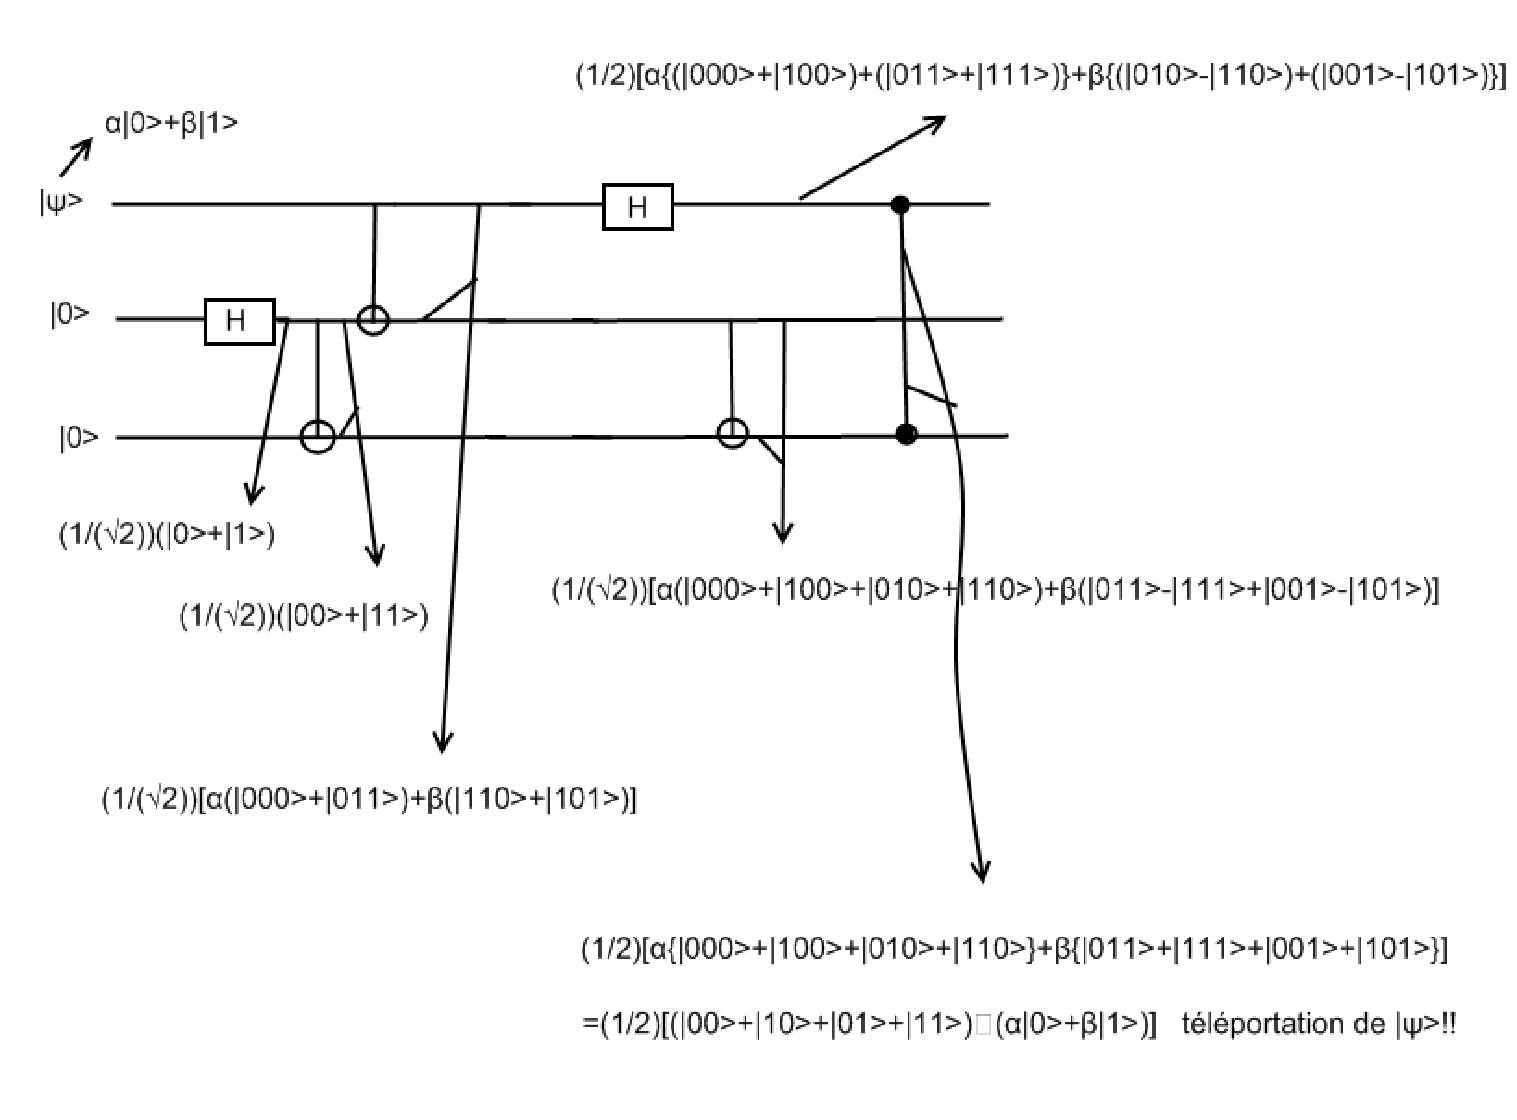
\includegraphics[scale=.6]{graphics/Interpolation_Sol.pdf}%
\caption{Méthode graphique de résolution du circuit intraportation.}%
\label{fig:methode1}%
\end{figure}

\begin{remark}
Si on applique 2 portes \texttt{W} aux 2 premiers qubits de cet état final, on
obtient l'état $\ket{00}$ qui co\"{\i}ncide avec l'état initial, hormis la
permutation des qubits.
\end{remark}

\item Méthode 2: du circuit, on a les 6 matrices $8\times8$ suivantes (de gauche
à droite):
$U_1=I_2\otimes \mathtt{W}\otimes I_2$; $U_2=I_2\otimes \mathtt{CNOT}$;
$U_3=\mathtt{CNOT}\otimes I_2$; $U_4=\mathtt{W}\otimes I_2\otimes I_2$;
$U_{5}=I_2\otimes \mathtt{CNOT}$; $U_{6}=CZ(1,3).$%

\begin{equation}
	\begin{split}
U_{6}U_{5}U_4U_3U_2U_1\ket{\psi00} &  =\frac
{1}{\sqrt{2}}U_{6}U_{5}U_4U_3U_2(\ket{\psi00}+\ket{\psi10}) \\
&  =\frac{1}{\sqrt{2}}U_{6}U_{5}U_4U_3(\ket{\psi00}+\ket{\psi11}) \\
&  =\frac{1}{2}U_{6}U_{5}U_4(\alpha\ket{000}+\beta\ket{110} +\alpha\ket{011}
+\beta\ket{101}) \\
&  =\frac{1}{2}U_{6}U_{5}[\alpha\{(\ket{000}+\ket{100})+(\ket{011}+\ket{111})\} \\
&  +\beta\{(\ket{010} -\ket{110})+(\ket{001} -\ket{101})\}]\\
&  =\frac{1}{2}U_{6}[\alpha(\ket{000} +\ket{100}+\ket{010} +\ket{110}) \\
&  +\beta(\ket{011} -\ket{100}+\ket{001}-\ket{101})]\\
&  =\frac{1}{2}[(\ket{00}+\ket{10}+\ket{01}+\ket{11})(\alpha\ket{0} +\beta
\ket{1})] \\
&  =[\frac{1}{\sqrt{2}}(\ket{0} +\ket{1})]\otimes[\frac{1}{\sqrt{2}}
(\ket{0} +\ket{1})]\otimes\ket{\psi}
\end{split}
\end{equation}

Une mesure des 2 premières sorties dans $\{\ket{0},\ket{1} \}$ donnent
aléatoirement les bits classiques.

\end{enumerate}

\subsection{Téléportation d'une paire EPR}

\begin{enumerate}
\item \textbf{Action de} \texttt{W}(2)
\begin{equation}
	\frac{1}{2}[\alpha(\ket{00}-\ket{01})+\beta(\ket{10} +\ket{11})]
(\ket{000}+\ket{111})]
\end{equation}

\item\textbf{Action de} \texttt{CX}(2,3)
\begin{equation}
	\frac{1}{2}[\alpha\{\ket{00000} +\ket{00111} -\ket{01100} -\ket{01011}\}
+\beta\{\ket{10000} +\ket{10111}+\ket{11100} +\ket{11011}\}  ]
\end{equation}

\item\textbf{Action de} \texttt{W}(2)
\begin{equation}
\begin{split}
&\frac{1}{2\sqrt{2}}[\alpha\{(\ket{00000}+\ket{01000})+(\ket{00111}+\ket{00111})
-(\ket{00100} -\ket{01100})-(\ket{00011} -\ket{01011})\}\\
&  +\beta\{(\ket{10000} +\ket{11000})+(\ket{10111} +\ket{11111})+(\ket{10100}
-\ket{11100})+(\ket{10011} -\ket{01011})\}]
\end{split}
\end{equation}
\item\textbf{Action de} \texttt{CX}(3,4)
\begin{equation}
\begin{split}
&\frac{1}{2\sqrt{2}}[\alpha\{\ket{00000} +\ket{01000} +\ket{ 00101} +\ket{01101}
-\ket{00110} +\ket{01110} -\ket{ 00011} +\ket{01011}\} \\
& +\beta\{\ket{10000} +\ket{11000} +\ket{10101} +\ket{11101} +\ket{ 10110}
-\ket{11110} +\ket{ 10011} -\ket{11011}\} ]
\end{split}
\end{equation}

\item\textbf{Action de} \texttt{CZ}(2,4)
\begin{equation}
\begin{split}
&\frac{1}{2\sqrt{2}}[\alpha\{ \ket{00000} +\ket{01000} +\ket{ 00101}
+\ket{01101} -\ket{ 00110} -\ket{01110} -\ket{ 00011} -\ket{01011}\} \\
& +\beta\{\ket{10000} +\ket{11000} +\ket{10101} +\ket{11101} +\ket{ 10110}
+\ket{11110} +\ket{ 10011} +\ket{11011}\} ]
\end{split}
\end{equation}

\item\textbf{Action de} \texttt{CX}(3,5)
\begin{equation}
\begin{split}
& \frac{1}{2\sqrt{2}}[\alpha\{ \ket{00000} +\ket{01000} +\ket{ 00100}
+\ket{01100} -\ket{ 00111} -\ket{01111} -\ket{ 00011} -\ket{01011}\} \\
& +\beta\{\ket{10000} +\ket{11000} +\ket{10100} +\ket{11100} +\ket{ 10111}
+\ket{11111} +\ket{ 10011} +\ket{11011}\} ]
\end{split}
\end{equation}

\item\textbf{Action de} \texttt{CX}(5,4)
\begin{equation}
\begin{split}
& \frac{1}{2\sqrt{2}} [\alpha\{\ket{00000} +\ket{01000} +\ket{00100}
+\ket{01100} -\ket{ 00101} -\ket{01101} -\ket{ 00001} -\ket{01001}\} \\
& +\beta\{\ket{10000} +\ket{11000} +\ket{10100} +\ket{11100} +\ket{ 10101}
+\ket{11101} +\ket{ 10001} +\ket{11001}\} ]
\end{split}
\end{equation}

\item\textbf{Action de} \texttt{CX}(4,1)
\begin{equation}
\begin{split}
& \frac{1}{2\sqrt{2}}[\alpha\{ \ket{00000} +\ket{01000} +\ket{ 00100}
+\ket{01100} -\ket{ 00101} -\ket{01101} -\ket{ 00001} -\ket{01001}\} \\
& +\beta\{\ket{10010} +\ket{11010} +\ket{10110} +\ket{11110} +\ket{ 10111}
+\ket{11111} +\ket{ 10011} +\ket{11011}\} ]
\end{split}
\end{equation}

\item\textbf{Action de} \texttt{W}(5)
\begin{equation}
\begin{split}
& \frac{1}{4}[\alpha\{(\ket{ 00000} +\ket{00001})+(\ket{01000}
+\ket{01001})+(\ket{ 00100} +\ket{00101})+(\ket{ 01100} +\ket{01101}) \\
& -(\ket{00100} -\ket{00101}) -(\ket{01100} +\ket{01101})
-(\ket{00000} -\ket{00001}) -(\ket{01000} -\ket{01001}) \}\\
& +\beta\{(\ket{10010} +\ket{ 10011})+(\ket{11010} +\ket{ 11011})+(\ket{10110}
+\ket{ 10111})+(\ket{11110} +\ket{ 11111}) \\
& +(\ket{10110} -\ket{10111}) +(\ket{11110} -\ket{11111})
+(\ket{10010} -\ket{10011}) +(\ket{11010} -\ket{11011}) \}]\\
& =\frac{1}{2}[\alpha\{\ket{00001} +\ket{01001} +\ket{00101} +\ket{01101}\}
+\beta\{\ket{10010} +\ket{11010} +\ket{10110} +\ket{11110}\} ]
\end{split}
\end{equation}

\item\textbf{Action de} \texttt{CX}(5,1)
\begin{equation}
\begin{split}
& \frac{1}{2}[\alpha\{ \ket{10001} +\ket{11001} +\ket{ 10101} +\ket{11101}\}
  +\beta\{ \ket{10010} +\ket{11010} +\ket{ 10110} +\ket{11110}\}] \\
& =\frac{1}{2}\ket{1} (\ket{00} +\ket{10} +\ket{01}+\ket{11})(\alpha\ket{01}
+\beta\ket{10}) \\
& =\ket{1} \otimes\frac{1}{\sqrt{2}}(\ket{ 0} +\ket{1})\otimes\frac{1}
{\sqrt{2}}(\ket{0} +\ket{1}) \otimes(\alpha\ket{01}+\beta\ket{ 10})
\end{split}
\end{equation}
\end{enumerate}

La paire EPR est téléportée!!

\subsection{Transformée de Fourier Quantique}

En vertu de
\begin{equation}
\mathtt{R}_2=\ket{0}\bra{0}+i\ket{1}\bra{1},\,
\mathtt{R}_3=\ket{0}\bra{0}+e^{\frac{\pi i}{4}}\ket{1}\bra{1},
\end{equation}
on a à la sortie de chaque fil du circuit:
\begin{figure}[ptbh]
\[
\Qcircuit @C=1em @R=1.em {
\lstick{\ket{1}} & \gate{W} & \gate{R_2} & \gate{R_3} & \qw & \qw & \qw & \qw
& \rstick{\frac{1}{\sqrt{2}}(\ket{0}-e^{\frac{\pi i}{4}}\ket{1})}  \qw \\
\lstick{\ket{0}} & \qw & \ctrl{-1} & \qw & \gate{W} & \gate{R_2} & \qw & \qw &
\rstick{\frac{1}{\sqrt{2}}(\ket{0}+i\ket{1})}  \qw \\
\lstick{\ket{1}} & \qw & \qw &\ctrl{-2} &\qw & \ctrl{-1} &\gate{W} & \qw &
\rstick{\frac{1}{\sqrt{2}}(\ket{0}-\ket{1})}  \qw
}
\]
\caption{Circuit implémentant la Transformation de Fourier Quantique (QFT) de
$\ket{101}$.}
\label{fig:solQFT3}
\end{figure}

On en déduit que la Transformée de Fourier Quantique (QFT) de $\ket{101}$ est
\begin{equation}
 \begin{split}
&\frac{1}{\sqrt{2^3}}(\ket{0}-e^{\frac{\pi i}{4}}\ket{1})\otimes
(\ket{0}+i\ket{1})\otimes(\ket{0}-\ket{1})\\
&=\frac{1}{\sqrt{2^3}}(\ket{000}-\ket{001}+i\ket{010}-i\ket{011}-e^{\frac{\pi
i}{4}}(\ket{100}-\ket{101}+i\ket{110}-i\ket{111}))\\
&=\frac{1}{\sqrt{2^3}}(\ket{0}-\ket{1}+i\ket{2}-i\ket{3}-e^{\frac{\pi i}{4}}
(\ket{4}-\ket{5}+i\ket{6}-i\ket{7}))
\end{split}
\end{equation}
